\section{Orbit integration}\label{sec:orbit}

\subsection{Three ways to integrate an orbit}\label{sec:orbit-paths}

\orb\ instances are set up and integrated as before, but an \orb\ instance whose
initial condition is a backend array, or whose potential carries a
backend parameter, is integrated in one of two new ways, depending on
what is to be differentiated. The first integrates the equations of
motion inside the backend, with the backend's own ODE solver:
\diffrax\ \citep{Kidger2021} for \jax, with an eighth-order
Dormand--Prince method, and \texttt{torchdiffeq} \citep{Chen2018} or
\torchode\ \citep{LienenGunnemann2022} for \torch, with a fifth-order method.
The equations of motion are those of \galpy's \cc\ integrators,
evaluated in rectangular coordinates through the backend force layer,
and the default tolerances are $10^{-12}$. Because the whole integration
is then a backend program, everything that enters it can be
differentiated: the initial condition, the potential's parameters, the
integration times. $N$ orbits are integrated in a single solve along a
batch axis, with per-orbit time grids if desired, and the solve runs on
a GPU when the initial conditions do. This is the path to use for
derivatives with respect to the parameters of the potential, 
as in the following example:
\begin{code}
def final_R(b):
    o= Orbit(jnp.asarray(ic))
    pp= PlummerPotential(amp=1.,b=b)
    o.integrate(ts,pp,method='diffrax')
    return o.R(ts[-1])
dR_db= jax.grad(final_R)(0.6)
\end{code}
and under \torch:
\begin{code}
b= torch.tensor(0.6,requires_grad=True)
o= Orbit(torch.as_tensor(ic))
pp= PlummerPotential(amp=1.,b=b)
o.integrate(torch.as_tensor(ts),pp,method='torchode')
o.R(ts[-1]).backward() # b.grad = dR/db
\end{code}
Second derivatives are available under \jax\ by selecting the direct
adjoint through the \texttt{inbackend\_kwargs} keyword, and
\texttt{jax.vmap} over initial conditions works, with one caveat
discussed below. \figurename~\ref{fig:orbitsens} displays the simplest
use of these derivatives: the sensitivity of an orbit to its initial
conditions as a function of time, which the solver's derivative gives
for free and which finite differences confirm, and a Gauss--Newton fit
of the launch velocity of an orbit to a target end point using the
Jacobian of the integration, which converges quadratically to machine
    precision in a handful of iterations.

\begin{figure*}[t!]
  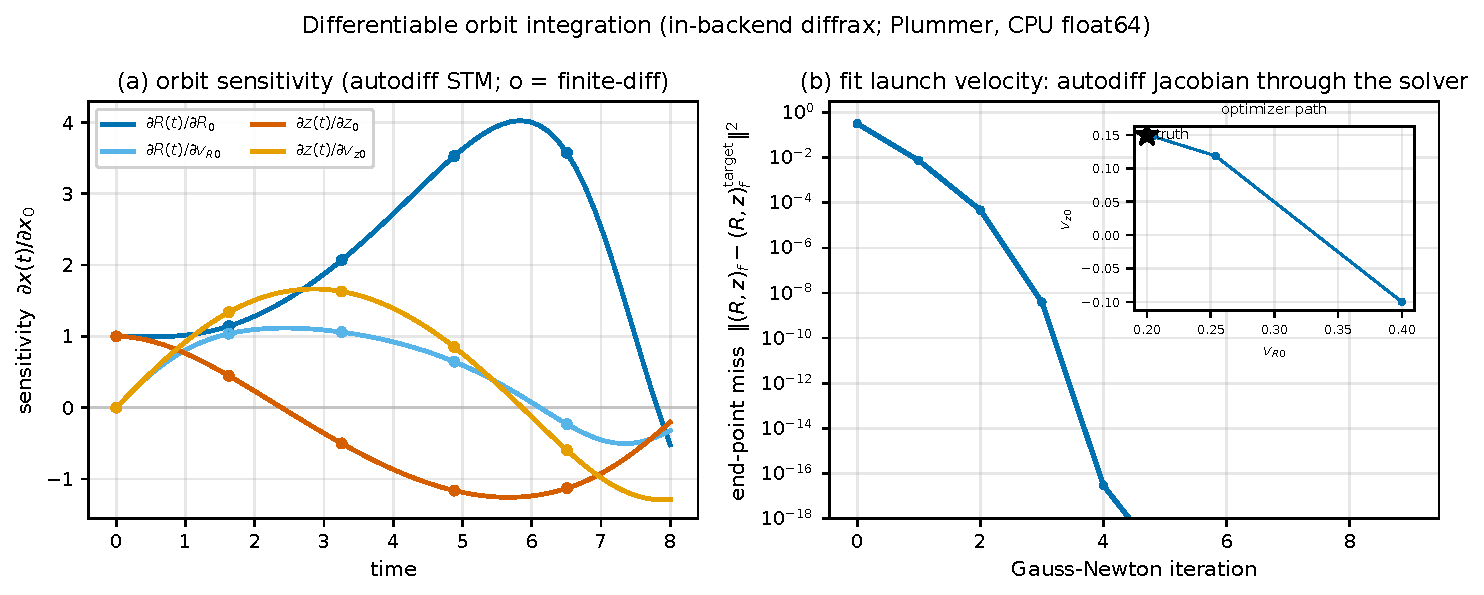
\includegraphics[width=\textwidth,clip=]{../figures/g7_orbit_sensitivity/g7_orbit_sensitivity.pdf}
  \caption{Derivatives of an in-backend orbit integration. Left: the
    sensitivities $\partial R(t)/\partial R_0$, $\partial R(t)/\partial v_{R,0}$,
    $\partial z(t)/\partial z_0$, and $\partial z(t)/\partial v_{z,0}$ of an
    orbit in a Plummer potential by reverse-mode differentiation through
    the \diffrax\ solve (lines) and by central finite differences
    (circles). Right: the squared distance between the end point of the
    orbit and a target as the launch velocity $(v_{R,0},v_{z,0})$ is
    fit by Gauss--Newton iterations on the Jacobian of the integration;
    the inset shows the path of the fit. The derivative through the
    solver agrees with the finite differences, and the fit that uses it
    converges in a handful of iterations.}\label{fig:orbitsens}
\end{figure*}

The second way uses \galpy's compiled \cc\ integrators, which are much
faster than a solver that runs inside \jax\ or \torch\ on a CPU (for a
single orbit in the Milky-Way model \texttt{MWPotential2014}, 
about ten times faster than the
\diffrax\ solve and a hundred times faster than \texttt{torchdiffeq}),
but which are opaque to automatic differentiation. What they can provide is the derivative of the
orbit with respect to its initial condition, through the variational
equations that \galpy\ integrates alongside the orbit in \cc\
(\appendixname~\ref{app:dxdv}). When a \galpy\ orbit with a backend
initial condition is integrated with a \cc\ method, the \cc\ integrator
returns both the orbit and the state-transition matrix
$\vec{M}(t) = \partial \vecw(t)/\partial \vecw(0)$, and a custom
derivative rule tells the backend that the derivative of the orbit with
respect to the initial condition is $\vec{M}$; the reverse-mode
derivative of any function of the orbit is then a single product of
$\vec{M}^T$ with the cotangent, without a second call to \cc. For a
six-dimensional orbit and a Runge--Kutta method, the six columns of
$\vec{M}$ are integrated together with the orbit as a 42-component
state; for the symplectic methods, the deviation vectors are propagated
through the same drift and kick steps as the orbit. The derivative is
exact to the precision of the solver: \figurename~\ref{fig:icjacobian}
compares the state-transition matrix of a Milky-Way orbit over 3\,Gyr
from the \cc\ variational equations with reverse-mode automatic
differentiation through
\diffrax\ and through \texttt{torchdiffeq} and with finite differences
of independently integrated orbits, and the four agree to a few parts in
$10^{10}$. In code, nothing marks the difference between the two paths except the
method:
\begin{code}
def end_point(ic):
    o= Orbit(ic)
    o.integrate(ts,MWPotential2014,
                method='dop853_c') # C + variational
    return jnp.stack([o.R(ts[-1]),o.z(ts[-1])])
M= jax.jacrev(end_point)(jnp.asarray(ic)) # STM rows
\end{code}
and a batch of orbits is differentiated with \texttt{jax.vmap},
\begin{code}
Ms= jax.vmap(jax.jacrev(end_point))(ics) # ics: (N,6)
\end{code}
This path gives derivatives with respect to the initial
conditions only, and to first order only; the variational equations do
not carry derivatives with respect to the parameters of the potential,
which must come from the in-backend solve.

\begin{figure*}[t!]
  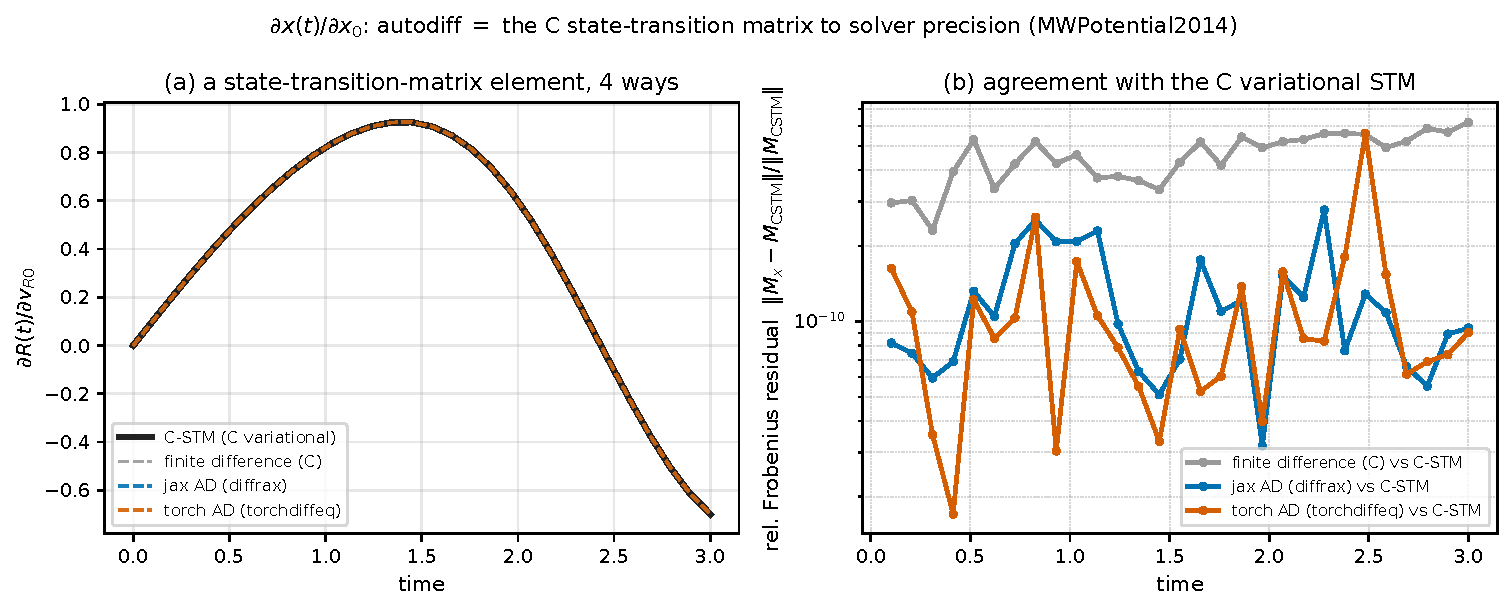
\includegraphics[width=\textwidth,clip=]{../figures/g16_icjacobian_precision/g16_icjacobian_precision.pdf}
  \caption{The derivative of an orbit with respect to its initial
    condition, in four ways. For a Sun-like orbit in \texttt{MWPotential2014}
    integrated for 3\,Gyr, the left panel shows one element of the
    state-transition matrix, $\partial R(t)/\partial v_{R,0}$, from the
    \cc\ variational equations, from a finite difference of the \cc\
    orbit, and from reverse-mode automatic differentiation through the
    \diffrax\ and \texttt{torchdiffeq} solvers. The right panel shows the
    relative Frobenius norm of the difference between each of the
    latter three and the variational result; all agree to a few parts in
    $10^{10}$.}\label{fig:icjacobian}
\end{figure*}

\galpy\ chooses between the two automatically. An \orb\ whose
initial condition is being differentiated---a traced \jax\ array or a
\torch\ tensor that requires a gradient---and that is integrated with
a \cc\ method, in a potential that has \cc\ second derivatives, with
non-traced times and non-traced potential parameters, uses the \cc\
integrator and its variational equations. In every other case in
which something is differentiated, in particular whenever a potential
parameter is traced or when the integration is to run on a GPU, the
in-backend solver is used, under the name \texttt{method='diffrax'},
\texttt{'torchode'}, or \texttt{'torchdiffeq'}, which can also be
requested directly. When nothing is being differentiated, that is, for
a concrete backend initial condition, a \cc\ method integrates in
\cc\ as before, without the variational equations, and only its result
is a backend array; this is not a third way of integrating but the old
one, and it means that a backend initial condition costs nothing until
it is differentiated. The pure-\python\ integrators of \galpy\
(\texttt{method='odeint'}, the \python\ leapfrog, and so on) are not
routed at all: given a backend initial condition they integrate in
\numpy\ and return a backend array that is not differentiable, with a
warning.

After integration, the orbit's methods work as before on backend
arrays: positions and velocities at the integration times or, by
interpolation with an in-backend spline, between them; energies and
angular momenta; peri- and apocenter radii and maximum height, both
from the integrated orbit and analytically through the action--angle
code of \sectionname~\ref{sec:aa} \citep{MackerethBovy2018}; and the transformations to observed
coordinates. Initializing an orbit from observed coordinates with
backend arrays works as well, such that a derivative with respect to a
star's distance or proper motion is available.

\subsection{Backend symplectic integrators for many orbits}\label{sec:orbit-leapfrog}

The in-backend solvers of \sectionname~\ref{sec:orbit-paths} are
adaptive Runge--Kutta methods: accurate, but expensive, because a step
of \diffrax's eighth-order Dormand--Prince method evaluates the force
thirteen times, and, as discussed in
\sectionname~\ref{sec:orbit-limitations}, their adaptive steps
complicate the derivative of a batch of orbits. For large batches of
orbits in a smooth potential, where modest precision suffices and the
cost is dominated by the force evaluations, a symplectic integrator
with a fixed step is the better tool: it evaluates the force once per
step, its energy error oscillates without a secular drift, it keeps
little state per orbit, and its fixed steps make the derivative of a
batch straightforward. \galpy\ therefore also integrates inside the
backends with a kick-drift-kick leapfrog with a constant step,
\texttt{method='leapfrog\_jax'} and \texttt{method='leapfrog\_torch'},
as for example in the following:
\begin{code}
o= Orbit(jnp.asarray(ics)) # ics: (N,6)
o.integrate(ts,MWPotential2014,method='leapfrog_jax',
            inbackend_kwargs={'nsteps':8000})
\end{code}
The same route provides backend versions of the fourth- and
sixth-order symplectic integrators \citep{Yoshida1990,Kinoshita1991}
of \galpy's \cc\ library, \texttt{method='symplec4\_jax'} and
\texttt{'symplec6\_jax'} (and their \torch\ twins), which evaluate the
force three and seven times per step and agree with their \cc\
counterparts at the same step to rounding; they are the better choice
when more than a few digits are wanted: for the batch of disc orbits of
\sectionname~\ref{sec:orbit-speed}, 450 sixth-order steps over 2\,Gyr
(3150 force evaluations) reach the worst-case accuracy of the adaptive
Dormand--Prince solve at tolerances of $10^{-8}$, which takes about 250
steps (3250 force evaluations).
The leapfrog is second order: its error falls by a factor of four per
halving of the step, and in a static potential its energy error
oscillates without the secular drift that a non-symplectic
second-order method with the same steps shows; we verified both for a
batch of 2000 orbits in \texttt{MWPotential2014} with a moving
satellite and the acceleration of a non-inertial frame, against the
\cc\ integrator. For reverse-mode
derivatives, the steps are grouped into blocks under the backend's
checkpointing (\texttt{jax.checkpoint} or \texttt{torch.utils.checkpoint}),
such that the derivative stores the state at the start of each block and
the states within one block, about $2\sqrt{N_\mathrm{steps}}$ states
rather than $N_\mathrm{steps}$: for $10^5$ orbits and 8000 steps in
\texttt{MWPotential2014}, the compiled \jax\ derivative needs 1.4\,GB of
temporary memory instead of 39\,GB. The derivatives agree with
Richardson-extrapolated central differences of the same integration to
$10^{-10}$, and the \jax\ and \torch\ versions agree with each other to
$2\times10^{-14}$. An initial condition in single precision is
integrated in single precision throughout, including the times and the
forces, which matters on GPUs with a low double-precision rate
(\sectionname~\ref{sec:orbit-speed}). Forces that do not derive from a
potential, such as dynamical friction or the Coriolis force of a
rotating frame, which \galpy\ marks with the \texttt{isConservative}
attribute, raise an error, because the closing kick would evaluate
them at the half-step velocity and the method would then converge only
at first order. As a second-order method, the leapfrog needs small steps
to be precise: for $10^4$ disc orbits integrated for 0.36\,Gyr, 1000
leapfrog steps (1000 force evaluations) give a worst-case position
error of $3\times10^{-4}$ (in units of $R_0$), while 250 Dormand--Prince
steps (3250 force evaluations) give $4\times10^{-7}$. The leapfrog is
therefore the method of choice when the force is expensive to evaluate
and modest precision suffices, the sixth-order integrator when the
orbits share a timescale and precision matters, and the adaptive
Runge--Kutta solvers remain the choice for batches that mix
timescales.

\subsection{Variational equations and chaos}\label{sec:orbit-dxdv}

The variational equations that the \cc\ state-transition matrix relies
on were part of \galpy\ for planar orbits since 2011; as part of this
work, we extended them to three-dimensional orbits, to all of the \cc\
integrators including the symplectic ones, to one-dimensional orbits,
and to dissipative, velocity-dependent forces, and we released them in
\galpy\ \flag{v1.12}. \appendixname~\ref{app:dxdv} gives the equations
and the checks that we applied to them. Their user-facing form is
\texttt{Orbit.integrate\_dxdv}, which integrates an orbit together with a
deviation vector or with the full state-transition matrix, and
\texttt{Orbit.lyapunov}, which computes the largest Lyapunov exponent, or
the spectrum, by the renormalization method of \citet{Benettin1980a,Benettin1980b},
for example as
\begin{code}
o= Orbit([0.8,0.3,0.75,0.,0.2,0.])
o.integrate_dxdv([1.,0.,0.,0.,0.,0.],ts,
                 MWPotential2014,method='dop853_c')
o.getOrbit_dxdv() # the deviation along the orbit
o.lyapunov(ts,MWPotential2014,method='dop853_c',
           renorm_every=10)
\end{code}
For
example, for the H\'enon--Heiles potential at $E=1/8$, the exponent of a chaotic orbit
converges into the range quoted in the literature while that of a
regular orbit at the same energy decays as $\ln t/t$
(\figurename~\ref{fig:lyapunov}). Like the variational equations
themselves, these are \numpy\ and \cc\ features that do not require
the backends: they accept backend initial conditions, but run on the
CPU, return \numpy\ arrays, and are not differentiable.

\begin{figure*}[t!]
  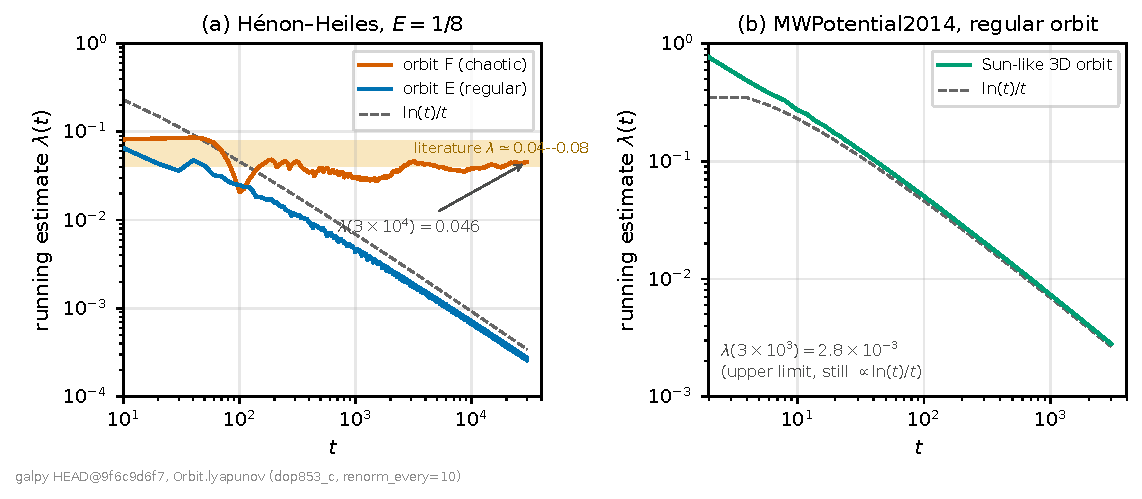
\includegraphics[width=\textwidth,clip=]{../figures/g10_lyapunov/g10_lyapunov.pdf}
  \caption{Largest Lyapunov exponent from \texttt{Orbit.lyapunov}, as a
    running estimate against time. Left: a chaotic and a regular orbit
    in the H\'enon--Heiles potential at $E=1/8$; the shaded band is the
    range of values in the literature for the chaotic orbit, and the
    dashed line is the $\ln t/t$ decay expected for a regular orbit.
    Right: a Sun-like orbit in \texttt{MWPotential2014}, which is
    regular. The estimate for the chaotic  H\'enon--Heiles orbit converges into the range
    found in the literature, while that for the regular orbit decays as
    expected.}\label{fig:lyapunov}
\end{figure*}

\subsection{Limitations}\label{sec:orbit-limitations}

In-backend orbit integration has a few limitations. 
By default, the derivative of an in-backend solve with respect to its
inputs differentiates through the solver's adaptive steps, which is
correct for a single orbit; when a batch of orbits is differentiated
under \texttt{jax.vmap}, however, the adaptive steps of one orbit depend
on the others and the derivative is wrong by several percent.
The remedy is to integrate with a fixed number of steps when
differentiating a batch, which \galpy\ does where it integrates batches
internally and which the user should do as well; \galpy\ warns when a
batch of orbits is differentiated through an adaptive in-backend
solve under \jax, where it can detect the derivative being taken, and
points at the fixed-step option. \texttt{torchdiffeq}
has no batching rule, such that a batch of orbits under \torch\ is a
\python\ loop unless \torchode\ is used. The eighth-order method of
\texttt{torchdiffeq} carries a gradient error of about $10^{-5}$ in its
backward pass, which is why \galpy\ uses its fifth-order method. Additionally, the
pure-\python\ integrators implemented in \galpy\ are not routed to the
backends (\sectionname~\ref{sec:orbit-paths}); they can run on a
backend under the forced mode of \sectionname~\ref{sec:design-choosing},
but are slow there, because each step is a separate set of array
operations, and we do not recommend it.
Finally, the \cc\ integrators cannot be used on a GPU at
all; their derivative rule runs the integration on the CPU.

\subsection{Speed}\label{sec:orbit-speed}

\figurename~\ref{fig:orbitspeed} compares the wall time of integrating
$N$ orbits for 2\,Gyr in \texttt{MWPotential2014} with the \cc\ integrator,
which parallelizes over orbits with OpenMP, on one core and on the 36
physical cores of the CPU node used in this work, and with the in-backend solvers on one CPU
core and on two GPUs. The absolute times depend on the specifics of the
problem, so we focus on the relative trends. On a single CPU core, the compiled \jax\
solve and the eager \torch\ solve cost about the same per orbit as the
\cc\ path for large batches, but they start from a floor of one to a
few seconds, set by compilation and kernel launches, that the \cc\ path
does not have, such that the \cc\ path is faster for up to a few
thousand orbits; the compiled solve additionally takes seconds to
compile, a cost that is paid once per shape of the problem. The \cc\
path is also the only one that makes use of more cores: its OpenMP loop
speeds up almost linearly to the 36 cores of our node for $10^4$ orbits
or more, eager \torch\ gains at most a factor of 3.5 (on 16 threads),
and compiled \jax, whose runtime keeps no more than a few cores busy,
gains nothing. The GPUs amortize a floor of half a second to a second
over the batch: the compiled \jax\ lines overtake one-core \cc\ at a
few hundred orbits and the \torch\ lines at a few thousand. The
consumer GPU, which executes double-precision arithmetic at one
thirty-second of its single-precision rate, never beats the 36-thread
\cc\ node with the adaptive solvers, while the H100 passes it at about
$10^4$ orbits and is 5 to 9 times cheaper per orbit for
$N\geq3\times10^5$. The
sixth-order symplectic integrator of
\sectionname~\ref{sec:orbit-leapfrog}, with the common step of that
section, is the cheapest in-backend route for this batch of disc
orbits, because its state per orbit is a fraction of the adaptive
solvers' and its steps are the same for every orbit: on one CPU core
it costs half of the adaptive \cc\ path, on the consumer GPU it beats
the 36-thread \cc\ node for $N\geq10^4$, which the adaptive solvers
cannot there, and on the H100 it is 3 to 7 times cheaper than the
adaptive solve on the same card and about 30 times cheaper than the
36-thread \cc\ node for $N\geq10^5$; for fewer
orbits, its compiled step loop is bound by its kernel launches, at
0.3--0.4\,s for the 450 steps on either GPU. The derivative of an orbit with respect to its
initial condition follows the same pattern
(\figurename~\ref{fig:icderivcost}): the \cc\ variational integrator
computes it fastest for a single orbit, by one to three orders of
magnitude over the backend solvers, and the GPU overtakes it at
batches of a few hundred orbits.

To gauge what GPU-native code could add, we also compiled \galpy's
\cc\ implementations of \texttt{MWPotential2014} and of its integrators
as a CUDA kernel that integrates one orbit per GPU thread; this is an
experiment and not part of \galpy. After restructuring the kernel, such
that the force is evaluated by a single out-of-line function and
threads pick up a new orbit when theirs is done, \texttt{dop853} on the
H100 is 4 to 11 times faster per orbit than \galpy's compiled \jax\
integrator on the same GPU and 30 to 90 times faster than the \cc\
integrator on the 36 cores of our CPU node (2.4\,$\mu$s per orbit
with a direct port of \galpy's \cc\ code and 0.9\,$\mu$s with special
functions rewritten for the GPU), while agreeing with the latter to
within its truncation error (\figurename~\ref{fig:orbitspeed}). The
kernel is limited by per-thread state: an adaptive eighth-order step
keeps $\approx$880\,B per orbit live, so few threads fit on each
multiprocessor. \galpy's sixth-order symplectic integrator with one
common step for the whole batch reaches the same accuracy with 15\%
fewer force evaluations and a fraction of the state, and runs another
3 to 4 times faster. These numbers hold for a smooth, cheap potential
and near-solar disc orbits with similar dynamical times, for which one
step suits every orbit; a batch that mixes very different timescales,
or has close encounters or a rapidly varying potential, has to step at
the rate of its fastest orbit, and there adaptive integration wins.
Such kernels are not differentiable, so they would complement the
backend integrators rather than replace them
(\sectionname~\ref{sec:conclusion}).

\galpy\ is not the only galactic-dynamics code that integrates orbits
with \diffrax: \texttt{galax} \citep{Starkman2026}, a re-implementation
of \texttt{gala} in \jax, does so by design, and comparing the two
checks that the cost of the in-backend solve is in the solver and the
potential rather than in the library around them. The green lines in
\figurename~\ref{fig:orbitspeed} show this comparison for the same
orbits, potential, and tolerances. When we make \texttt{galax} control
its step size per orbit, as \galpy\ does, the two codes take the same
time to within 13 per cent on both GPUs for batches of $10^5$ orbits or
more; for smaller batches, whose cost is dominated by fixed overheads,
they differ by up to a factor of 1.6, in opposite directions on the two
GPUs. In its default mode, \texttt{galax} integrates the whole batch as
one system with a single step-size controller, whose error estimate is
the root-mean-square over all orbits, such that one sequence of steps
serves every orbit; this is cheaper per orbit for large batches, by a
factor of two to three, at the price of an error control that holds
only in the batch-averaged sense and that depends on which orbits
happen to be in the batch. \galpy\ keeps the per-orbit control.

\begin{figure*}[t!]
  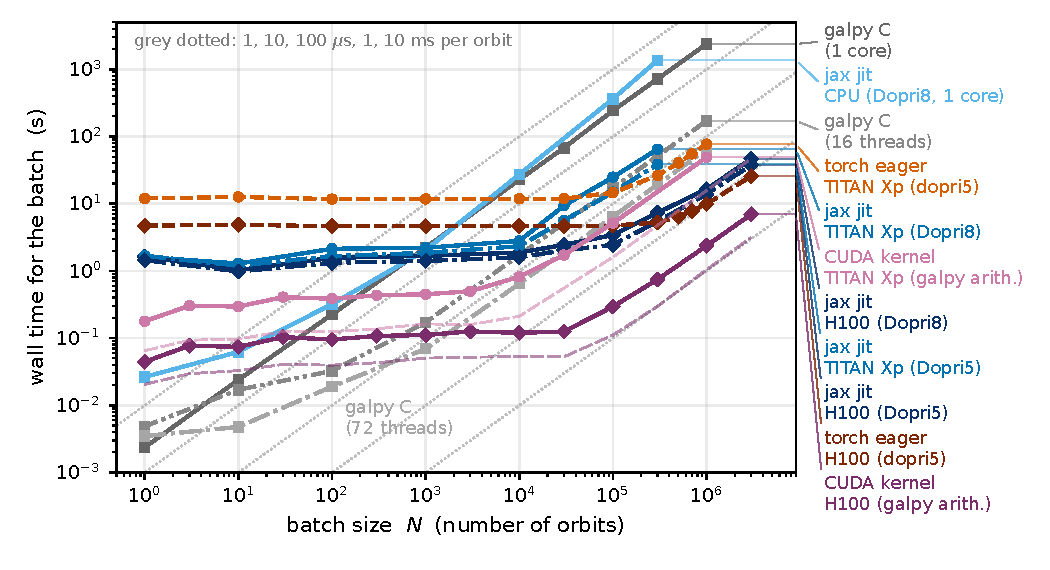
\includegraphics[width=\textwidth,clip=]{../figures/g12_inbackend_orbit_gpu/g12_inbackend_orbit_gpu.pdf}
  \caption{Wall time for integrating $N$ orbits for 2\,Gyr in
    \texttt{MWPotential2014} with relative and absolute tolerances of
    $10^{-8}$, on (a) the CPU, (b) the TITAN~Xp, and (c) the H100; each
    label repeats the style of its line. Grey: \galpy's \cc\ integrator
    \texttt{dop853\_c}, which parallelizes over orbits with OpenMP, on
    one core, 16 threads, and the 36 physical cores of the node; the
    latter is repeated in the GPU panels for reference. Blue: the
    in-backend \diffrax\ solve under \jax, compiled, with the
    eighth-order method that \galpy\ uses by default and with a
    fifth-order method that performs the same number of force
    evaluations as the \torch\ solve, and the in-backend sixth-order
    symplectic integrator (\texttt{symplec6\_jax}) with 450 common
    steps over the 2\,Gyr, the step at which its worst-case position
    error over the batch equals that of the adaptive solve. Orange and
    red: the eager \texttt{torchdiffeq}
    solve. Green: \texttt{galax} with its default batched step-size
    control and with per-orbit control as in \galpy. Purple: an
    experimental CUDA port of \galpy's \cc\ forces and \texttt{dop853}
    that integrates one orbit per GPU thread (not part of \galpy\ and
    not differentiable), with a direct port of \galpy's \cc\ code and
    with special functions rewritten for the GPU, including the copies
    between host and device, which keep these lines flat up to
    $N\approx10^4$. Light grey dotted lines mark a constant cost per
    orbit, and the arrows point towards lower wall time.}\label{fig:orbitspeed}
\end{figure*}

\begin{figure*}[t!]
  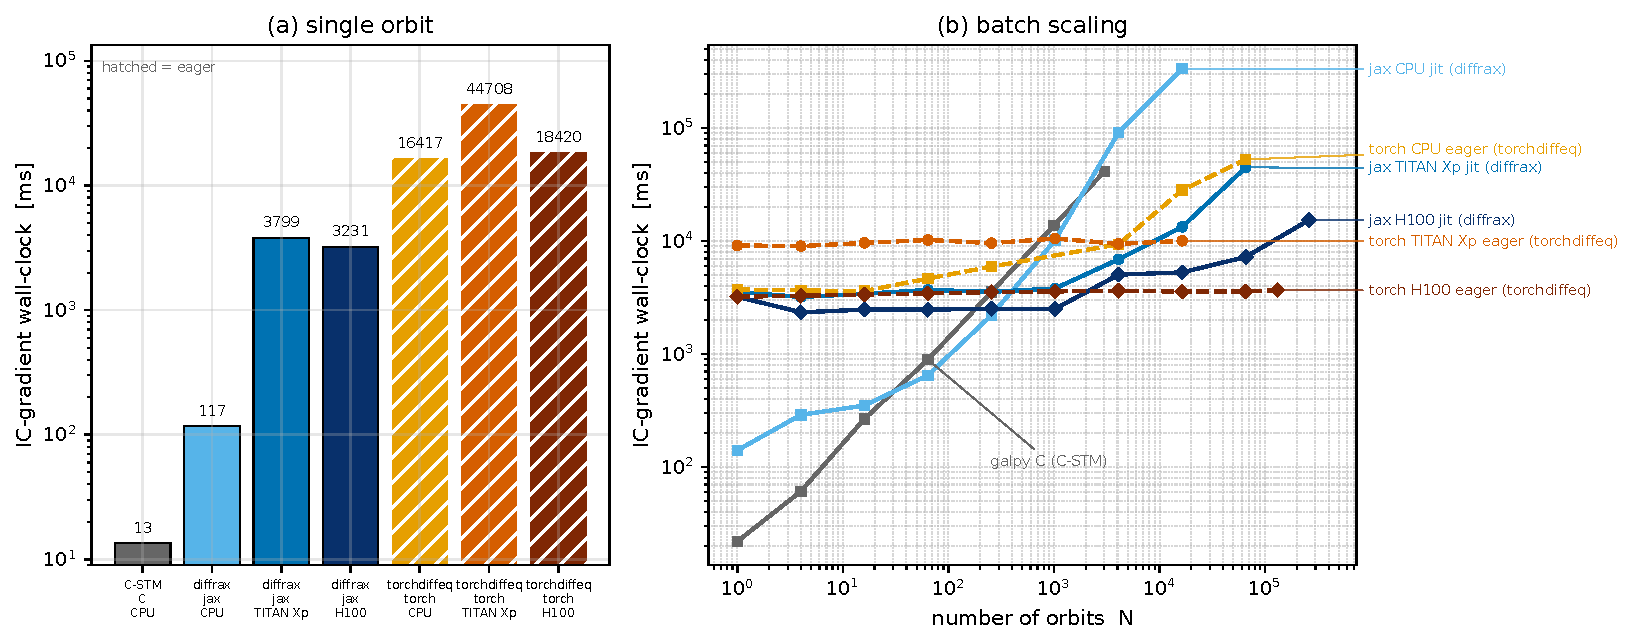
\includegraphics[width=\textwidth,clip=]{../figures/g15_icderiv_speed/g15_icderiv_speed.pdf}
  \caption{Cost of the derivative of an orbit with respect to its
    initial conditions, for a 2\,Gyr orbit in \texttt{MWPotential2014}.
    Left: wall time for a single orbit with the \cc\ variational
    integrator and by reverse-mode differentiation through the
    \diffrax\ and \texttt{torchdiffeq} solves on the CPU and the two
    GPUs; hatched bars are eager and solid bars compiled. Right: the same as a function of the
    number of orbits differentiated at once. The \cc\ variational
    integrator is the fastest way to obtain the derivative of a single
    orbit, while a GPU overtakes it for large batches. All CPU timings use
    one core.}\label{fig:icderivcost}
\end{figure*}

